% !TEX root = main.tex
\chapter{Design and simulation of the addressing setup}
The purpose of this thesis work was to design and build the addressing setup for the already existing experiment. In this chapter we discuss the design and the implementation of such setup. The design is a crucial part of the work, there are several requirements that have to be met in order to achieve the proper needed functionality. In the first section, the requirements are presented together with an overview of the design idea. In the setup an objective was already present, ad the choice of an AOD was already made. Hence, we discuss this components as given. The rest of the setup was simulated with the software Zemax, which was used to find the optimal optical components and their placement.
\section{Addressing system overview and requirements}
Addressing systems have already been developed and employed in experiments successfully. Different techniques are available: the main idea is to focus a laser beam tighter than ion-ion separation and steer it. In  Innsbruck calcium ions have been addressed in this way, where the steering was achieved with an AOD \cite{addressing}; Beam has also been steered with micro-electromechanical systems (MEMS) mirrors \cite{addressing3}. Another idea is to send a normal beam illuminating all the ions, but hiding those who are not addressed. This was done with Ytterbium atoms where by means of a inhomogeneous magnetic field the transition frequencies were shifted shielding selected ions \cite{addressing2}. \\
Our choice was to implement the already successful idea of Innsbruck with an AOD and improve it. The advantage of AODs is to have a fast switching time in the order of $\mu$s, that is used for fast switching between ions. A problem with the implementation of \cite{addressing} is however the fact that the AOD is placed right before the beam expander, this limits the addressing range, as the beam is likely to clip when it is steered on the edge of the AOD's bandwidth. This is the main problem that the new designed system, here implemented, wanted to address: exploiting the full capabilities of the AOD while maintaining a very tight focus.
Therefore, there are mainly two aspects to keep in mind, the focus spot and the addressing range.\\
The addressing setup should be able to address single ions in a string in order to generate single photons out of single ions via the already discussed Raman process. Ion separations, in the case of $^{40}\text{Ca}^+$, has been derived in section \ref{ionstrings}, for a trap frequency of 1 MHz is 5.6 $\mu$m. The setup must therefore be able to focus tightly a laser beam down to 1-2 $\mu$m. As seen in section \ref{sec_diffraction}, a tighter focus can obtained with a shorter wavelength, a bigger lens, or with shorter focal length. The focusing lens, a.k.a the objective, is shared with the imaging setup, and thus it is given, the focal length is therefore a constant in the problem. The wavelength is also a constant, as the Raman process happens only at 393 nm. This gives only one possibility left to tighten the focus, i.e. by making the beam as broad as possible at the objective input surface. Beam expansion can be achieved with a Galilean telescope, it take two lenses to form such Telescope, a concave Lenses to diverge a collimated beam and a convex lens to collimate the diverging beam. The combinations of these two lenses takes a collimated beam and expands it to another collimated beam. This expansion part is one of the two essential part of the addressing setup. The other part is related to addressing range. Not only, we want to focus the beam to a single ion, but we want to move the beam as well, such that it focuses on a different ion. Therefore, there is a requirement also on the range that can be addressed. This depends on the number of ions and their spacing, a good aim is to address tens of ions, this requires the ability to move the focus in one direction by 150-200 $\mu$m. Beam steering is possible with the use of an AOD, the detailed working principle of this device has been discussed in section \ref{theory_AOD}. Basically the angle of the output beam of the AOD changes as the driving frequency changes. However, the AOD must be placed far behind the objective to leave space for the beam expander, this implies a need to control and redirect the angle of the AOD's output beam to send it to the beam expander and later in the objective without any clipping. This task is accomplished with a pair of converging lenses, they refocus the collimated beam into the beam expander, beam then becomes wider, reaches the objective and it is focused on the ion. It is important to get the right lenses at the right distances, the objective has 5 different lenses inside and it works slightly differently from a normal lens. For instance, it does not focuses collimated blue light, but red. This means that the beam expander should not collimate completely the beam but rather expand it and leave it diverging, so that the objective can focus it at the right position.\\
The setup displayed in figure \ref{addressingsetup} also contains polarization optics. As discussed in section \ref{sec:ramanprocess}, Zeeman transitions are polarization sensitive, thus polarization control is required. The AOD is polarization sensitive, which means it requires a certain input polarization and outputs another particular polarization, that is the reason why half wave plate are before and after, and additional quarter wave plate is inserted before the objective to obtain circular polarized light. This placements means having a non standard plate, but if placed before in the optical path, the mirror and the beam splitter could alter the polarization. The choice of using a beam splitter is also peculiar, to separate light at different wavelength it is common choice to use a dichroic mirror, however the light in the imaging path is 397 nm, very close to the 393 nm light of the addressing setup. This would have meant using a very narrow dichroic, the alternative was to use a 90:10 beam splitter, where 90 \% of the light is transmitted and only 10 \%of the light is reflected. The addressing therefore loses 90 \% of the power on this splitter, but that is not a problem, since it is always possible to get more light out of the laser. Furthermore, this light is focused so tightly that even a small amount of light can excite the ions. On the other end, it is not really possible to get more scattered light from the ions, so 397 nm light and the imaging setup must be as efficient as possible, with 10 \% of losses, ions are still visible on the camera and on the PMT.

\begin{figure}
\centering
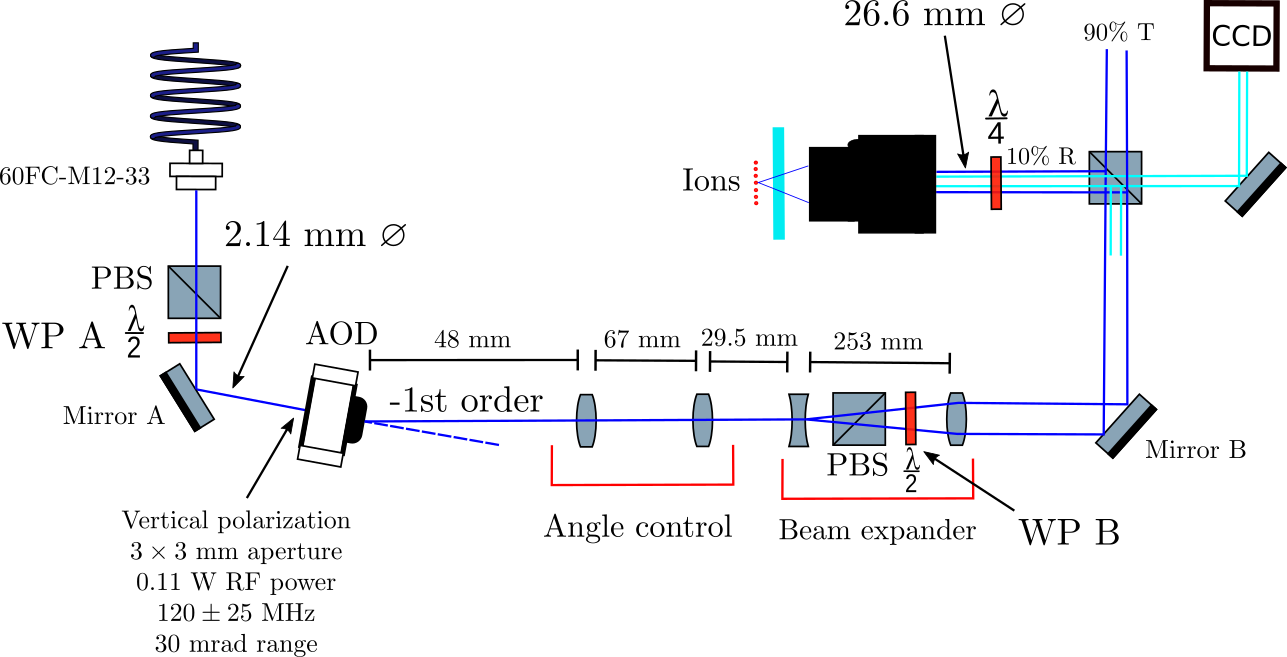
\includegraphics[width=\textwidth]{img/setup}
\caption{Setup scheme}
\label{addressingsetup}
\end{figure}

\section{Objective and AOD}
\label{sec:obj}
The objective used to focus the light was already present in the system and had to be taken as it is. It is a custom objective by Sill optics placed outside vacuum, the section is in figure \ref{objsection}. It contains 5 lenses inside a mechanical housing, the aperture is about 47 mm large in diameter.
This objective has different purposes, it was designed keeping in mind: imaging of ions, addressing with red light and addressing of blue light. The objective has to perform all three of this jobs fairly well, which means it has light transmission >90 \%, every lenses is AR coated, numerical aperture of NA = 0.3. Moreover, it is telecentric, which means that the focus spot should move perpendicularly to the optical axis if the beam is steered. Lastly it was also designed to take into consideration the fact that it is placed out of vacuum, the light after the objective has to go through a 6 mm fused silica viewport before entering the vacuum and after further 40 mm encounters the ions. The focal length of the objective is 54.07 mm at 729nm. The objective is also mounted on a 3 dimensional translational stage to allow for imaging and addressing calibration.
\begin{figure}[H]
     \centering
     \begin{subfigure}[b]{0.4\textwidth}
         \centering
         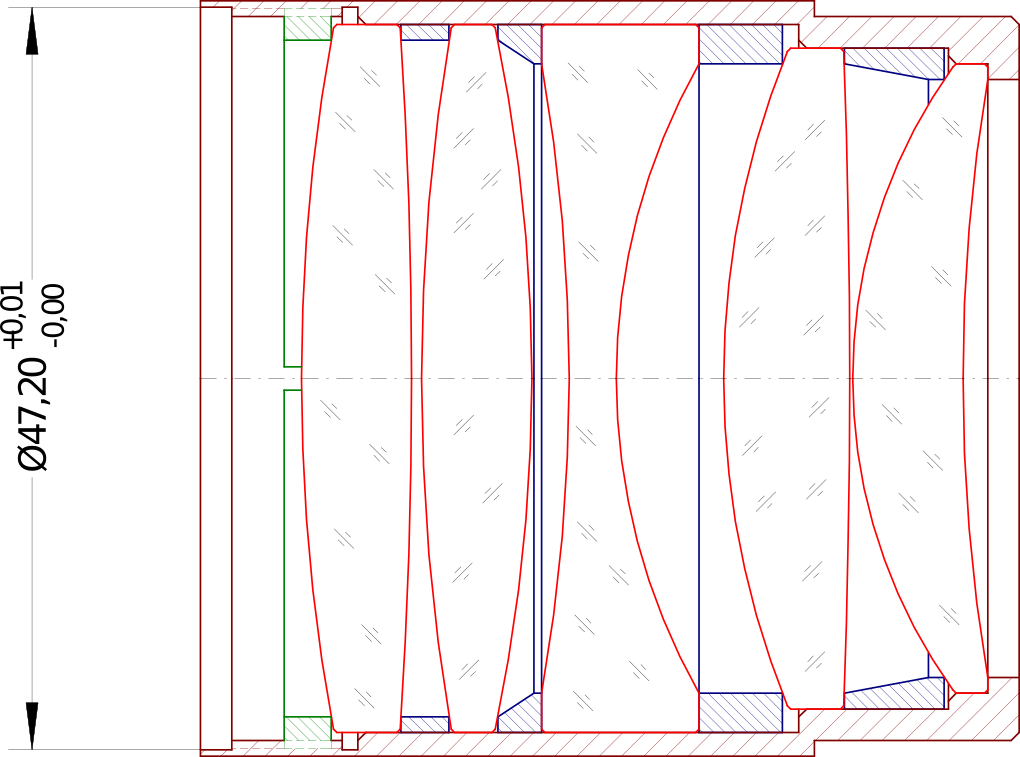
\includegraphics[width = \textwidth]{obj}
          \caption{Section of the custom objective, red parts are the lenses, while the rest is the housing.}
         \label{objsection}
     \end{subfigure}
     \hfill
     \begin{subfigure}[b]{0.55\textwidth}
         \centering
         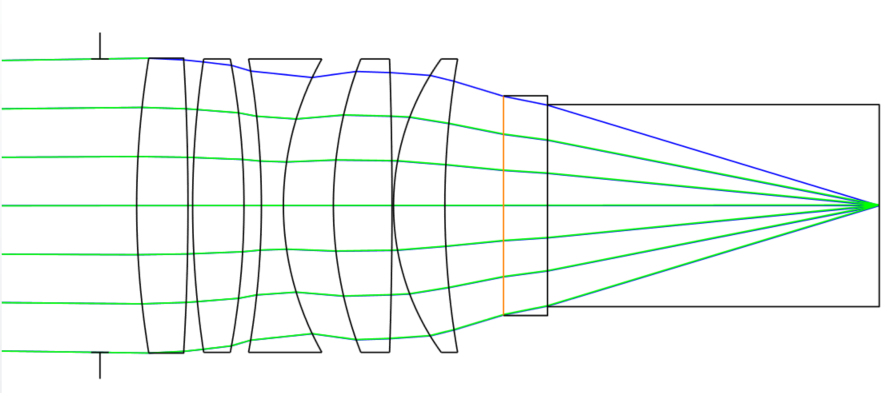
\includegraphics[width=\textwidth]{zeemaxobj}
         \vspace{1em}
         \caption{Zemax simulation of the objective. On the right, viewport and the vacuum chamber are also present.}
         %\label{fig:three sin x}

     \end{subfigure}
        \caption{}
      %  \label{fig:three graphs}
\end{figure}
The AOD is from Gooch \& Housego, model 4120-3. It has a specified central frequency of 120 MHz, with 50 MHz, bandwidth, so the driving frequency ranges from 95 to 145 MHz with a maximum RF power of 0.3 W. Therefore, the angle of deflection should be $\pm 0.86^{\circ}$ (:|).  In this bandwidth the diffraction efficiency should remain above 75 \% and have an average of 83 \%. Further light is lost as much as 3\% of due to insertion losses. The active aperture measures $3\times 3$ mm, and the polarization has to be horizontal when entering the AOD, while it gets rotated during diffraction, as the specified output polarization is vertical.

\section{Design simulation}
The setup in figure \ref{addressingsetup} has been simulated with the software Zemax. The simulation had the purpose of assessing the performance of the setup, i.e. checking the viability of the setup and see if it meets all requirements. It was also used to find the best lenses for building the setup and the best placement. Not everything was simulated, bu only the essential parts. This includes the four lenses, the objective, the viewport and the vacuum chamber. As there is no option to simulate an AOD, it was not taken in consideration, instead the simulation started at the output of the AOD as described below. Mirrors and beam splitters also do not alter drastically the optical path and therefore there was no need to simulate them.



\begin{figure}[H]
\centering
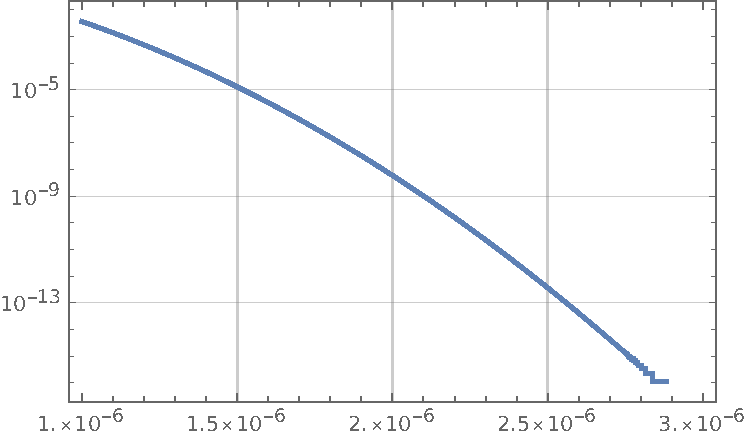
\includegraphics[width=\textwidth]{img/Plosses}
\caption{Losses on the compensation electrodes vs beam waist}
\end{figure}
\begin{figure}[H]
\centering
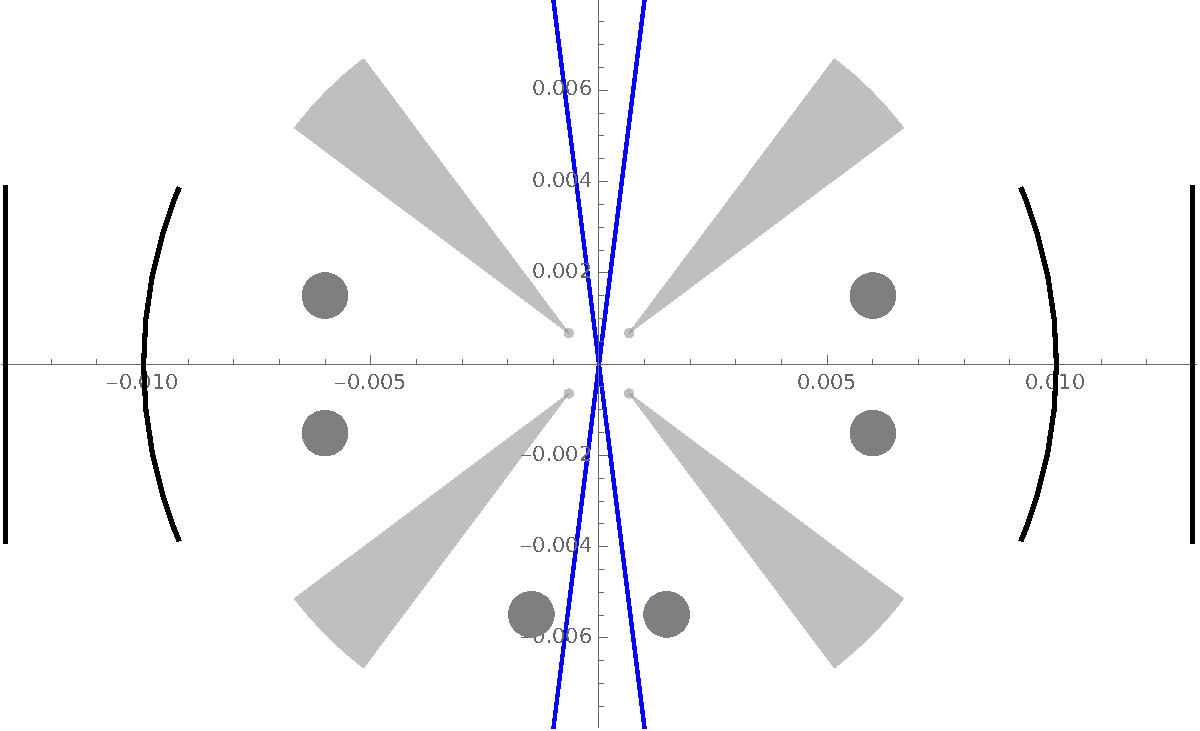
\includegraphics[width=\textwidth]{img/clipping}
\caption{Clipping on compensation electrodes}
\end{figure}

\section{Physical implementation}
- test setup
- picture
- alignment process
